\documentclass[11pt]{article}
\usepackage[margin=1in]{geometry}
\usepackage{amsmath, amssymb}
\usepackage{graphicx}
\usepackage{booktabs}
\usepackage{hyperref}
\usepackage{float}
\usepackage{enumitem}
\usepackage{caption}
\usepackage{subcaption}

% If images are in a figures/ subfolder, uncomment the next line:
% \graphicspath{{figures/}}

\title{\textbf{Predicting S\&P 500 Market Direction Using Machine Learning}}
\author{Eric Liu, Rithikesh Muddana \\ EE 344 --- Final Project}
\date{March 2026}

\begin{document}
\maketitle

% ===================================================================
\begin{abstract}
We apply multiple machine learning classifiers to the task of predicting whether the S\&P 500 index will close higher or lower on the next trading day. Our feature set combines historical price data (returns, moving averages, RSI, MACD, Bollinger Bands) with macroeconomic indicators (CBOE Volatility Index, 10-year Treasury yield, unemployment rate). We evaluate Logistic Regression, Random Forest, Gradient Boosting, and a feedforward neural network against three simple baselines using a strictly chronological train/validation/test split covering January 2022 through December 2025. On the held-out 2025 test set (250 trading days), Gradient Boosting achieved the highest ROC-AUC of 0.5174 and was the only model with precision above 61\%, while the Always-Up baseline achieved the highest F1 of 0.7310 due to the market's inherent upward bias. We conduct error analysis across VIX regimes, trend direction, and volatility levels, finding that models perform notably better during high-VIX and high-volatility periods.
\end{abstract}

% ===================================================================
\section{Introduction}
\label{sec:intro}

The S\&P 500 index tracks the performance of the 500 largest U.S.\ publicly traded companies and is widely regarded as the primary benchmark for the U.S.\ equity market. Predicting its daily direction---whether it will close up or down---is a classic challenge in quantitative finance.

From a machine learning perspective, this is a binary classification problem. The input features include historical price-derived indicators and macroeconomic variables. The target is a binary label: 1 if tomorrow's close exceeds today's close, and 0 otherwise.

Market movements are influenced by complex, nonlinear relationships between many variables, making this problem well-suited for ML approaches that can capture feature interactions that simple linear models miss. However, financial time series present unique challenges: temporal dependence, regime changes, and the ever-present risk of overfitting to noise.

We structure the project around three goals:
\begin{enumerate}
    \item Build a robust, leakage-free data pipeline that respects the chronological nature of the data.
    \item Compare multiple model families---linear, tree-based, and neural---against meaningful baselines.
    \item Analyze where and why models fail across different market conditions.
\end{enumerate}

% ===================================================================
\section{Data and Preprocessing}
\label{sec:data}

\subsection{Data Sources}

We use four datasets, all publicly available:

\begin{itemize}
    \item \textbf{S\&P 500 Index Historical Data} (Yahoo Finance): Daily OHLC prices from January 2022 to December 2025. This is our primary dataset and defines the time axis.
    \item \textbf{CBOE Volatility Index (VIX)} (FRED): Daily closing values of the VIX, which measures implied volatility from S\&P 500 options.
    \item \textbf{10-Year Treasury Yield} (FRED): Daily yield on the 10-year U.S.\ Treasury note, a key indicator of interest rate expectations.
    \item \textbf{Unemployment Rate} (Bureau of Labor Statistics via FRED): Monthly U.S.\ unemployment rate, reported with approximately a one-month lag.
\end{itemize}

The combined dataset contains 993 trading days. Figure~\ref{fig:eda} shows the S\&P 500 closing price, VIX, and macroeconomic indicators over the full period, along with the class distribution of up vs.\ down days.

\begin{figure}[H]
    \centering
    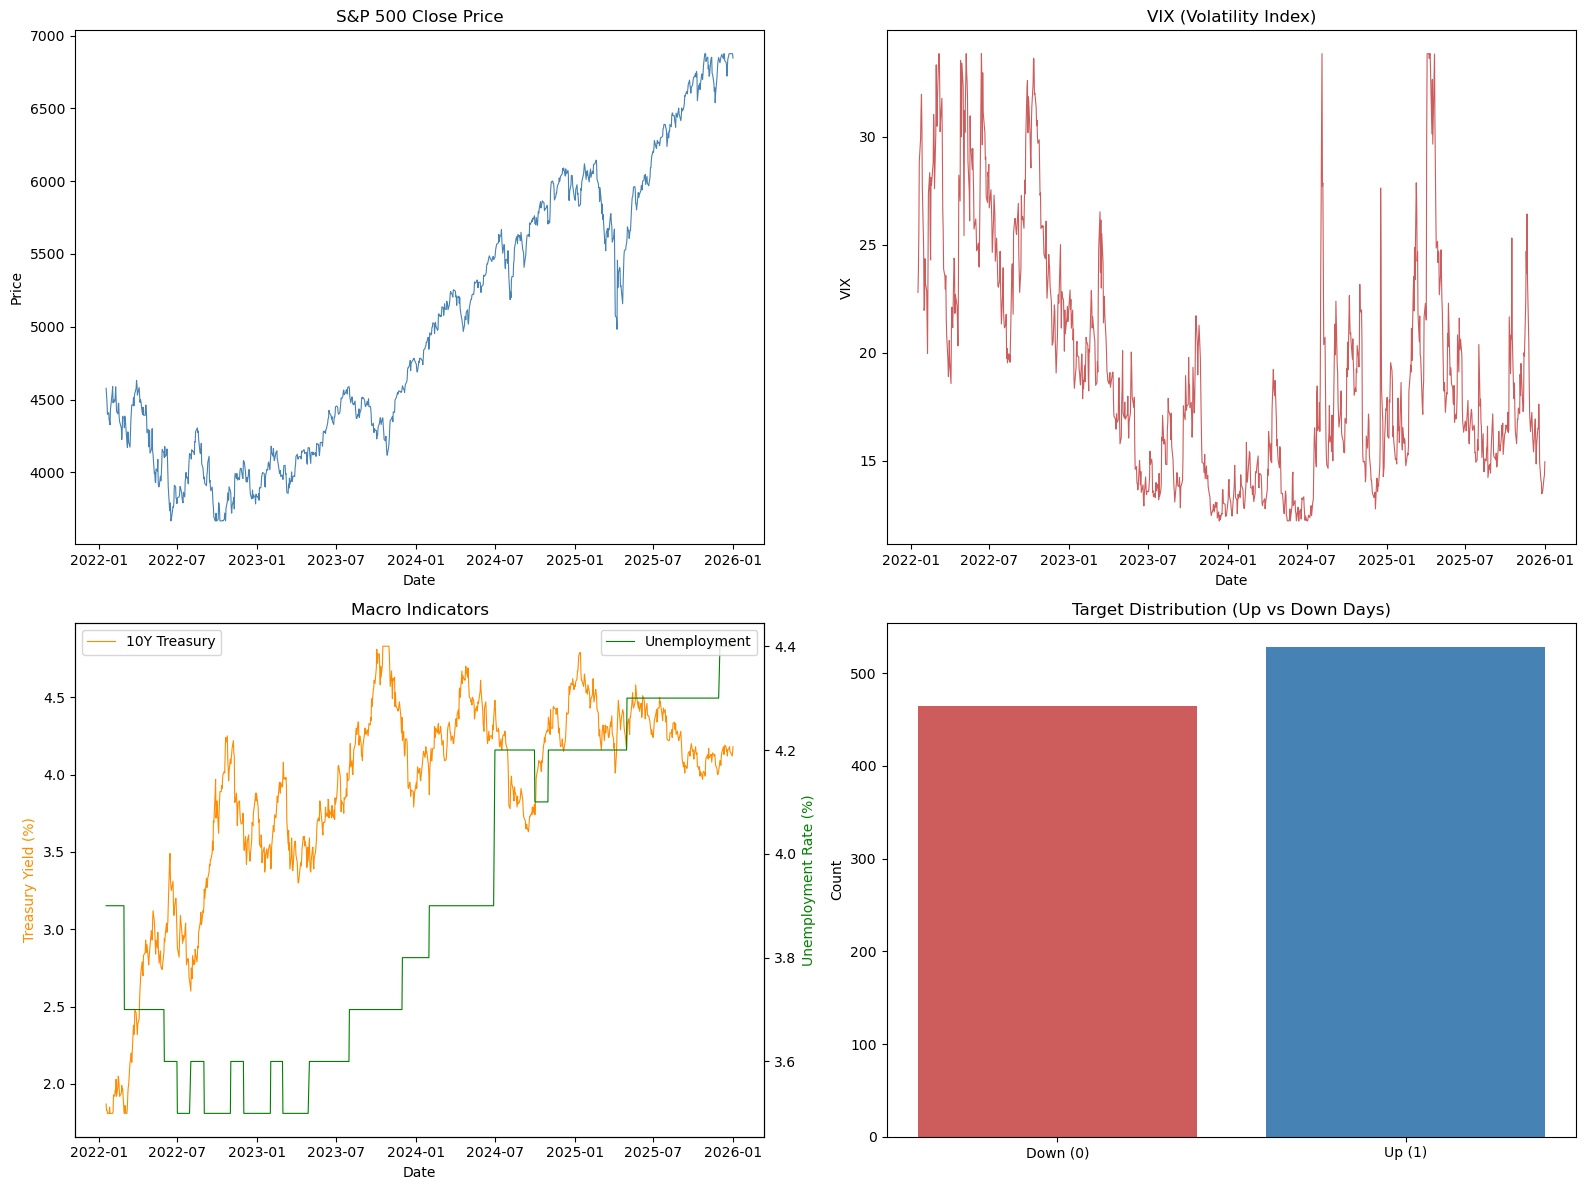
\includegraphics[width=\textwidth]{fig_eda_overview.png}
    \caption{Overview of the dataset. Top-left: S\&P 500 closing price. Top-right: VIX volatility index. Bottom-left: 10-year Treasury yield and unemployment rate. Bottom-right: class balance---528 up days (53.2\%) vs.\ 465 down days (46.8\%).}
    \label{fig:eda}
\end{figure}

\subsection{Data Alignment}

Since these datasets arrive at different frequencies, we establish explicit alignment rules:

\begin{itemize}
    \item \textbf{S\&P 500 and VIX} (daily): Direct merge on date.
    \item \textbf{Treasury Yield} (daily, with holiday gaps): Forward-filled to cover missing dates.
    \item \textbf{Unemployment Rate} (monthly): Forward-filled so that each trading day uses the most recently released figure. Since BLS releases unemployment data with roughly a one-month lag, this guarantees no look-ahead bias.
\end{itemize}

\subsection{Prediction Horizon}

We predict next-day close-to-close direction. On trading day $t$, we use all available information up to and including day $t$ to predict whether day $t+1$'s closing price will exceed day $t$'s closing price.

\subsection{Data Cleaning}

\begin{itemize}
    \item \textbf{Missing values}: Forward-fill for unemployment rate (monthly) and treasury yield (holiday gaps). VIX aligns directly.
    \item \textbf{Outlier treatment}: Winsorization at the 1st and 99th percentiles. Financial outliers are informative (e.g., crash days), so we cap rather than discard them.
\end{itemize}

\subsection{Feature Engineering}

We derive 30+ features from the raw data, organized into several categories:

\begin{itemize}
    \item \textbf{Returns and Lags}: Daily returns over 1, 3, 5, 10, and 20-day windows, plus 5 lagged daily returns.

    \item \textbf{Volatility}: 5-day and 20-day rolling standard deviation of returns, and their ratio.

    \item \textbf{Moving Averages and Crossovers}: Price relative to 5, 10, 20, 50, and 200-day SMAs, plus pairwise SMA crossover ratios (e.g., SMA5 vs.\ SMA20, SMA50 vs.\ SMA200).

    \item \textbf{RSI}: 14-day Relative Strength Index.

    \item \textbf{MACD}: 12/26 EMA difference, 9-day signal line, and histogram.

    \item \textbf{Bollinger Bands}: Percent B and band width relative to the 20-day SMA.

    \item \textbf{Intraday Features}: High-low range and open-close gap as fractions of the closing price.

    \item \textbf{Macro Indicators}: Treasury yield, unemployment rate, and VIX close (used directly as features).
\end{itemize}

All features use only information available at time $t$ for predicting $t+1$. Rolling windows are backward-looking by construction. The target label uses \texttt{shift(-1)} on the close price, ensuring no future data enters the feature set.

% ===================================================================
\section{Exploratory Data Analysis}
\label{sec:eda}

\subsection{Feature Correlations}

Figure~\ref{fig:corr} shows the correlation matrix across all model features. The target variable (next-day direction) has very low linear correlation with any individual feature---the strongest positive correlations are Treasury Yield ($r = 0.080$) and Unemployment Rate ($r = 0.075$), and the strongest negative correlations are VIX Close ($r = -0.056$) and 5-day volatility ($r = -0.054$). This is expected for daily market prediction: if any single feature were strongly predictive, the market would have already priced it in.

\begin{figure}[H]
    \centering
    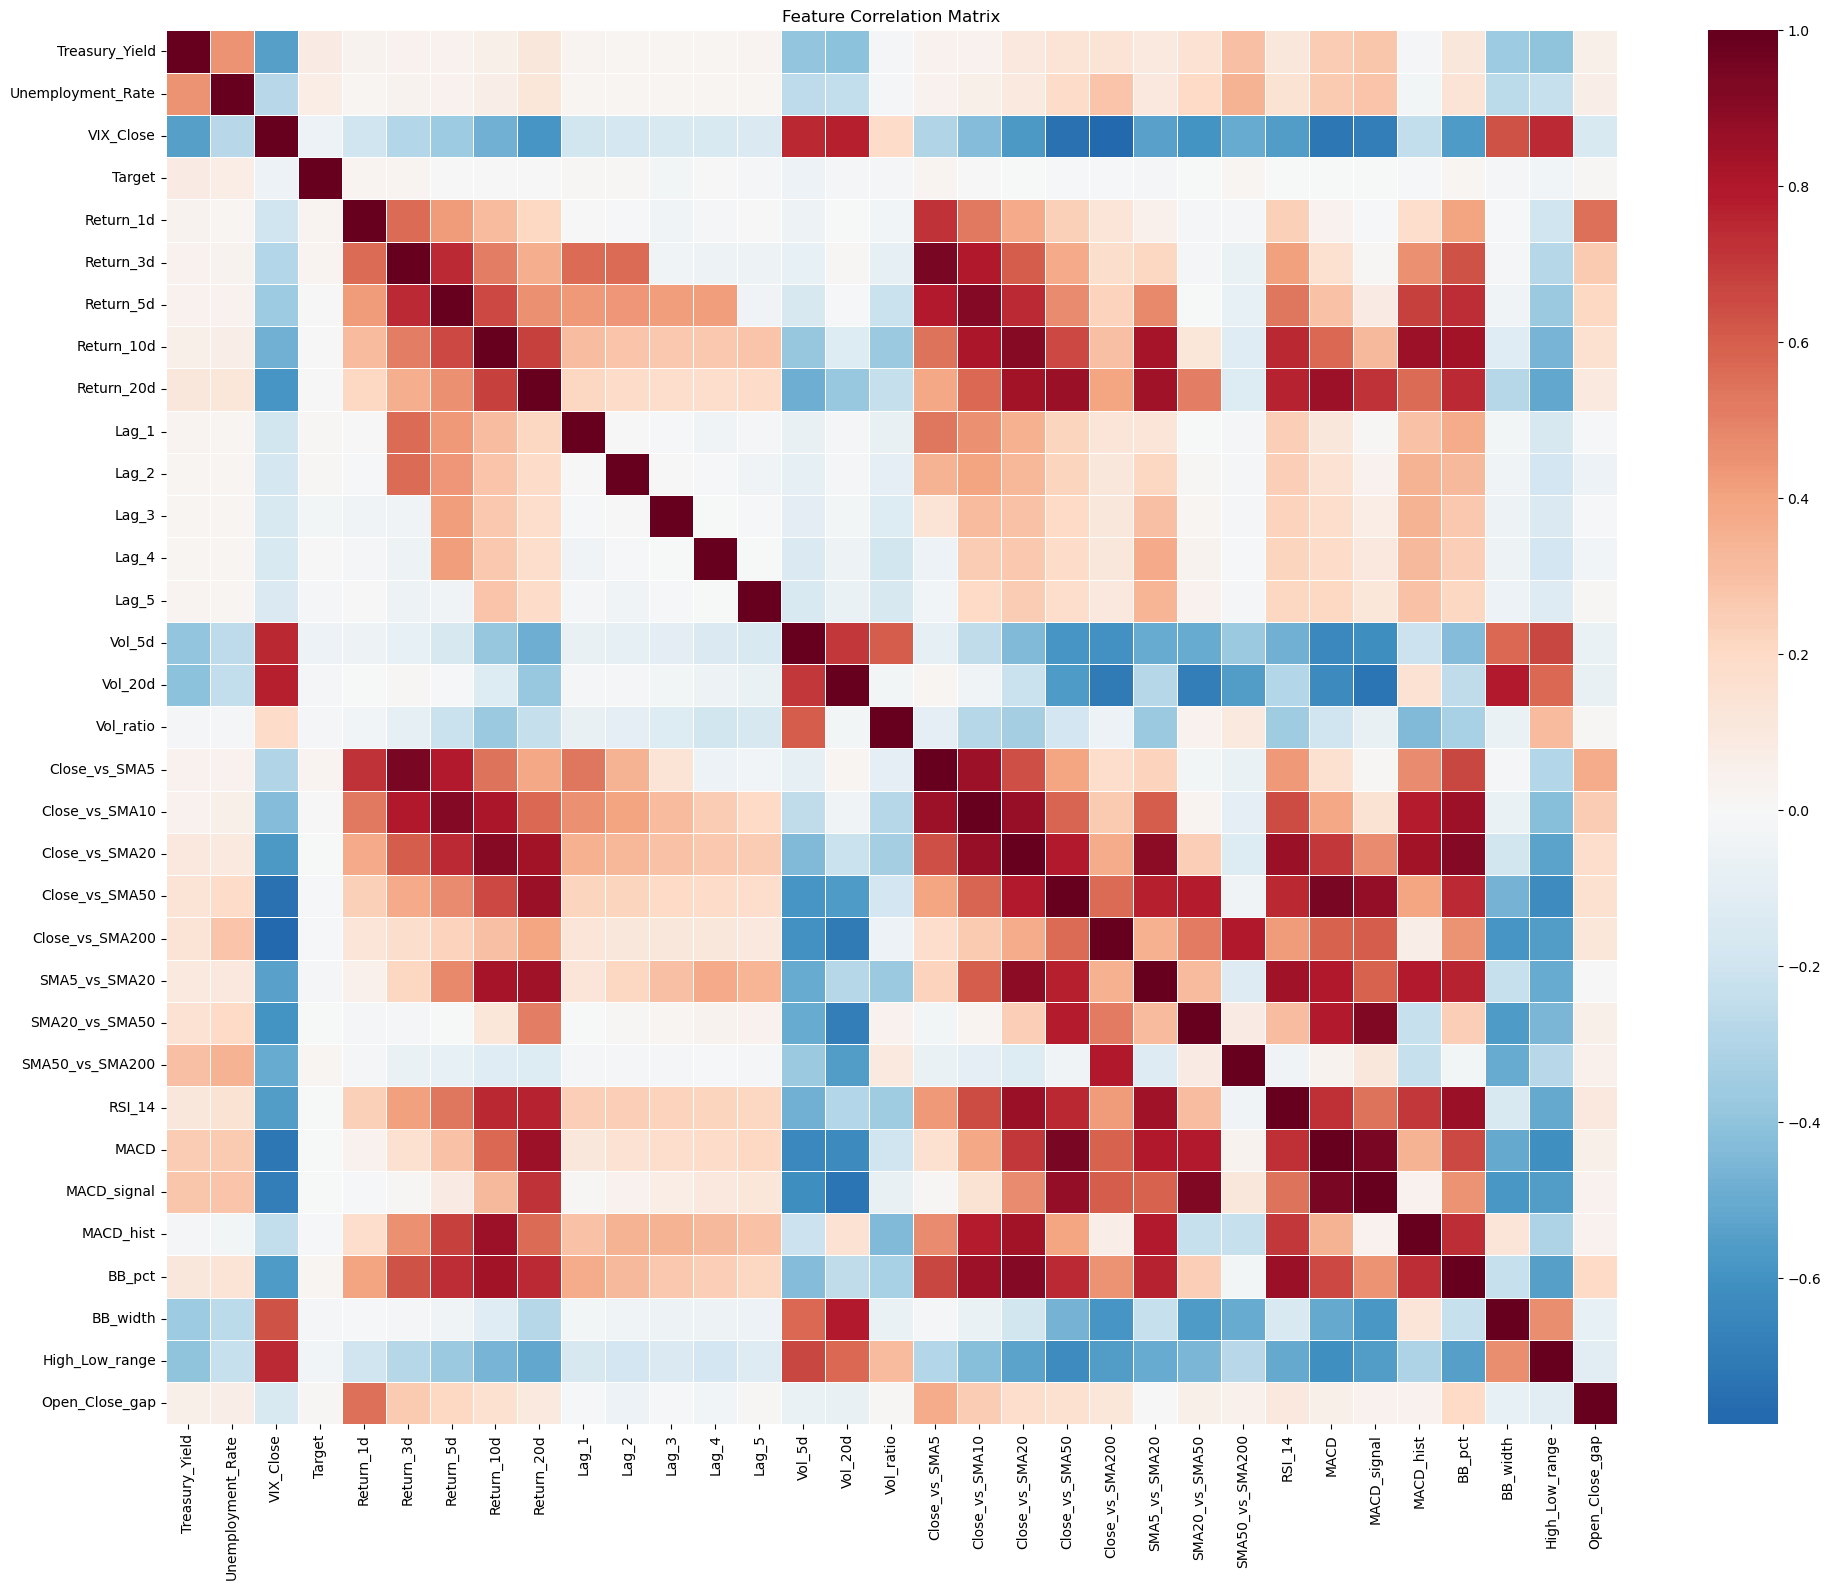
\includegraphics[width=\textwidth]{fig_correlation.png}
    \caption{Correlation matrix of all model features. Individual features have very weak linear correlation with the target (next-day direction), confirming that this is a hard prediction task.}
    \label{fig:corr}
\end{figure}

\subsection{Feature Distributions by Class}

Figure~\ref{fig:dist} shows the distribution of six key features split by target class (up vs.\ down days). The distributions overlap heavily for all features, further illustrating the difficulty of the classification task. Return\_1d and VIX\_Close show the most visible separation.

\begin{figure}[H]
    \centering
    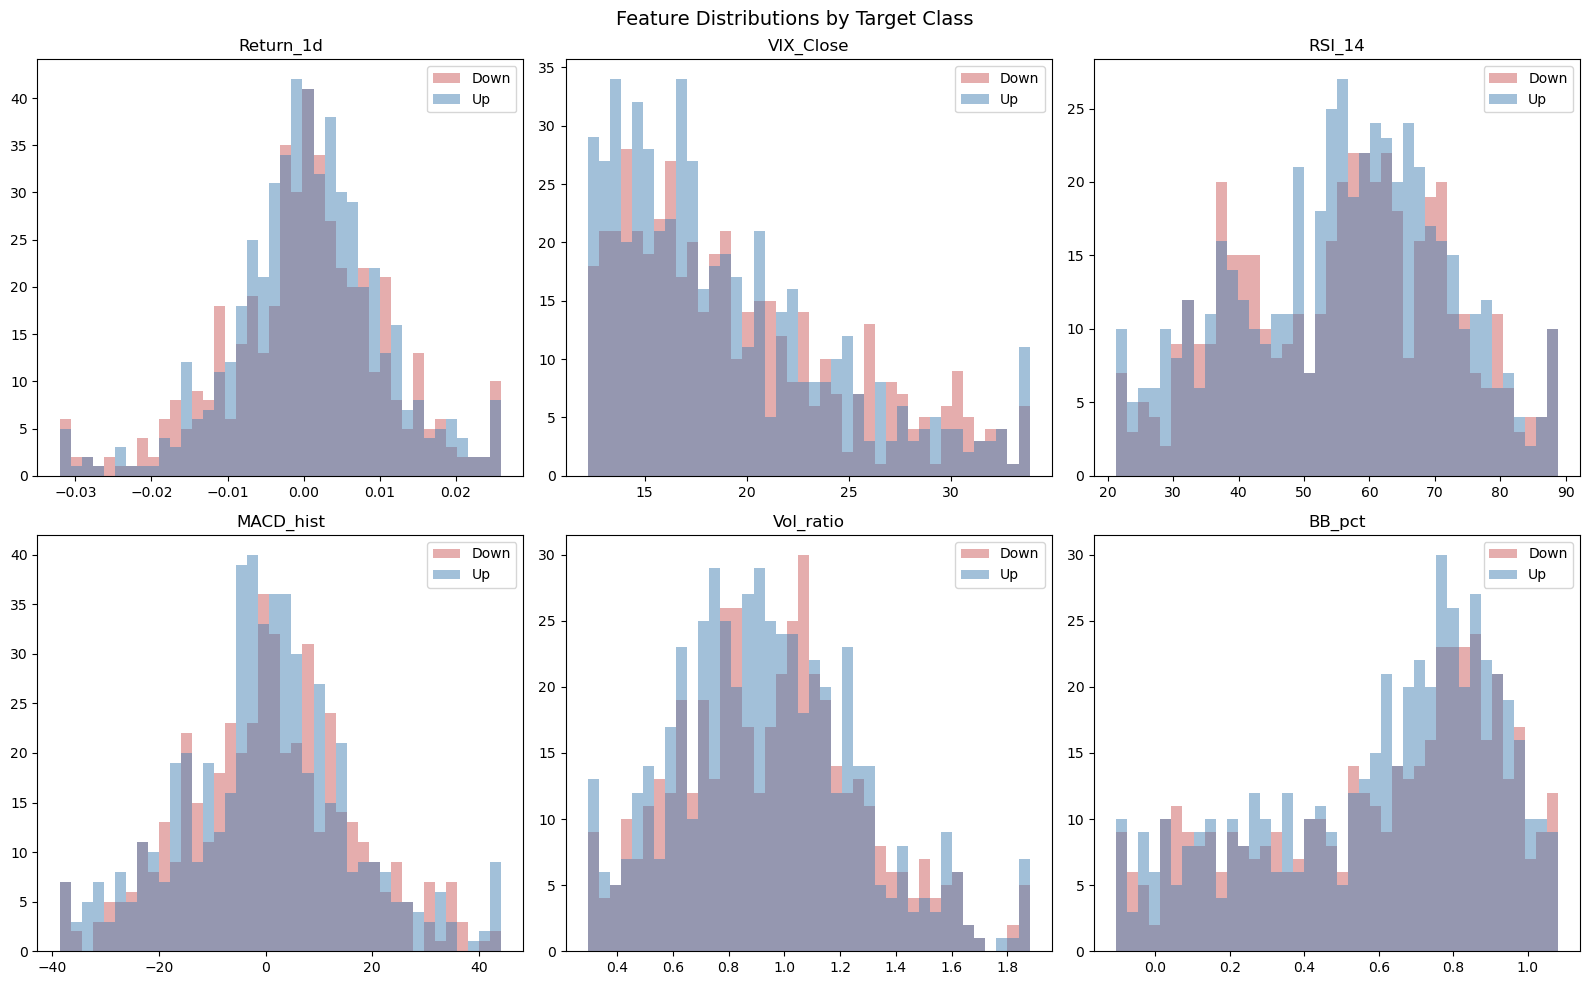
\includegraphics[width=\textwidth]{fig_feature_dist.png}
    \caption{Histograms of key features conditioned on target class. Blue = up days, red = down days. Heavy overlap across all features confirms the signal is weak at the individual feature level.}
    \label{fig:dist}
\end{figure}

% ===================================================================
\section{Methodology}
\label{sec:method}

\subsection{Train/Validation/Test Split}

We split the data chronologically---no random shuffling. The first $\sim$200 rows are dropped due to NaN values from the 200-day SMA warmup period, leaving 794 usable samples.

\begin{itemize}
    \item \textbf{Training set}: Nov 2022 -- Jun 2024 (416 samples, 53.8\% up)
    \item \textbf{Validation set}: Jul 2024 -- Dec 2024 (128 samples, 57.0\% up)
    \item \textbf{Test set}: Jan 2025 -- Dec 2025 (250 samples, 57.6\% up)
\end{itemize}

Features are scaled using \texttt{RobustScaler} fit only on training data to prevent information leakage.

\subsection{Baseline Models}

To establish a performance floor, we evaluate three baselines:

\begin{enumerate}
    \item \textbf{Always Up}: Predict class 1 (up) every day. Since 57.6\% of test days are up, this baseline achieves 57.6\% accuracy.
    \item \textbf{Same as Yesterday}: Predict that today's direction equals yesterday's actual direction.
    \item \textbf{Return-Only Logistic}: Logistic regression using only the previous day's return as input.
\end{enumerate}

\subsection{Machine Learning Models}

\subsubsection{Logistic Regression}
A linear classifier with $L_2$ regularization ($C = 1.0$, \texttt{max\_iter} = 1000). Serves as an interpretable model that uses the full feature set.

\subsubsection{Random Forest}
An ensemble of 200 decision trees (\texttt{max\_depth} = 10, \texttt{min\_samples\_leaf} = 10). Captures nonlinear feature interactions without extensive tuning.

\subsubsection{Gradient Boosting}
Sequential ensemble of 200 shallow trees (\texttt{max\_depth} = 4, \texttt{learning\_rate} = 0.05, \texttt{subsample} = 0.8). Generally the strongest off-the-shelf method for structured tabular data.

\subsubsection{Feedforward Neural Network}
A PyTorch MLP with architecture: Input $\to$ 64 (ReLU, Dropout 0.3) $\to$ 32 (ReLU, Dropout 0.2) $\to$ 1 (Sigmoid). Trained with Adam (\texttt{lr} = $10^{-3}$, \texttt{weight\_decay} = $10^{-4}$) and binary cross-entropy loss. Early stopping with patience of 15 epochs based on validation F1 score. The model stopped at epoch 24.

\subsection{Hyperparameter Tuning}

We tune the Gradient Boosting classifier using walk-forward (expanding window) cross-validation via \texttt{TimeSeriesSplit} with 5 folds on the combined train+validation set. The search space covers:
\begin{itemize}
    \item \texttt{n\_estimators}: \{100, 200, 300\}
    \item \texttt{max\_depth}: \{3, 4, 5\}
    \item \texttt{learning\_rate}: \{0.01, 0.05, 0.1\}
\end{itemize}

We evaluated 12 randomly sampled parameter combinations. The top 5 configurations are shown in Table~\ref{tab:cv}.

\begin{table}[H]
\centering
\caption{Walk-forward CV results (top 5 configurations by mean F1).}
\label{tab:cv}
\begin{tabular}{ccccc}
\toprule
\textbf{n\_estimators} & \textbf{max\_depth} & \textbf{learning\_rate} & \textbf{Mean F1} & \textbf{Std F1} \\
\midrule
100 & 3 & 0.01 & 0.5676 & $\pm$ 0.1011 \\
200 & 5 & 0.05 & 0.5602 & $\pm$ 0.0615 \\
300 & 5 & 0.01 & 0.5538 & $\pm$ 0.0443 \\
100 & 3 & 0.05 & 0.5534 & $\pm$ 0.0541 \\
200 & 3 & 0.01 & 0.5469 & $\pm$ 0.0657 \\
\bottomrule
\end{tabular}
\end{table}

The best configuration (\texttt{n\_estimators} = 100, \texttt{max\_depth} = 3, \texttt{learning\_rate} = 0.01) was retrained on the full train+validation set for final evaluation on the test set.

% ===================================================================
\section{Results}
\label{sec:results}

\subsection{Model Comparison}

Table~\ref{tab:results} presents the full comparison of all models on the held-out test set (250 trading days, Jan--Dec 2025).

\begin{table}[H]
\centering
\caption{Test set performance for all models, sorted by F1 score. Baselines are separated by a horizontal rule.}
\label{tab:results}
\begin{tabular}{lccccc}
\toprule
\textbf{Model} & \textbf{Accuracy} & \textbf{F1} & \textbf{Precision} & \textbf{Recall} & \textbf{ROC-AUC} \\
\midrule
Always Up            & 0.5760 & 0.7310 & 0.5760 & 1.0000 & ---    \\
Same as Yesterday    & 0.5040 & 0.5694 & 0.5694 & 0.5694 & ---    \\
Return-Only Logistic & 0.5320 & 0.6812 & 0.5605 & 0.8681 & 0.4892 \\
\midrule
Logistic Regression       & 0.5720 & 0.7206 & 0.5774 & 0.9583 & 0.4505 \\
Random Forest             & 0.5240 & 0.6246 & 0.5723 & 0.6875 & 0.4879 \\
Gradient Boosting         & \textbf{0.5480} & 0.5979 & \textbf{0.6131} & 0.5833 & \textbf{0.5174} \\
Gradient Boosting (Tuned) & 0.5240 & 0.6293 & 0.5706 & 0.7014 & 0.4942 \\
Neural Network (MLP)      & 0.5520 & 0.7021 & 0.5690 & 0.9167 & 0.4486 \\
\bottomrule
\end{tabular}
\end{table}

Several observations stand out:

\begin{itemize}
    \item The \textbf{Always-Up baseline} achieves the highest F1 (0.7310) because F1 rewards recall---predicting every day as ``up'' captures all true up days. This makes F1 alone misleading for this task.

    \item \textbf{Gradient Boosting} (untuned) achieves the best ROC-AUC (0.5174) and the highest precision (0.6131), meaning it is the most selective when predicting ``up.'' This is the only model with precision above 61\%.

    \item \textbf{Logistic Regression} and the \textbf{Neural Network} both have very high recall ($>$0.91) but low precision ($\sim$0.57), indicating they default to predicting ``up'' most of the time---behaving similarly to the Always-Up baseline.

    \item The \textbf{Same as Yesterday} baseline is the weakest at 50.4\% accuracy, confirming that simple momentum persistence does not hold at the daily level.
\end{itemize}

Figure~\ref{fig:comparison} shows bar charts comparing all models across accuracy, F1, and ROC-AUC. Baselines are shown in red, trained models in blue.

\begin{figure}[H]
    \centering
    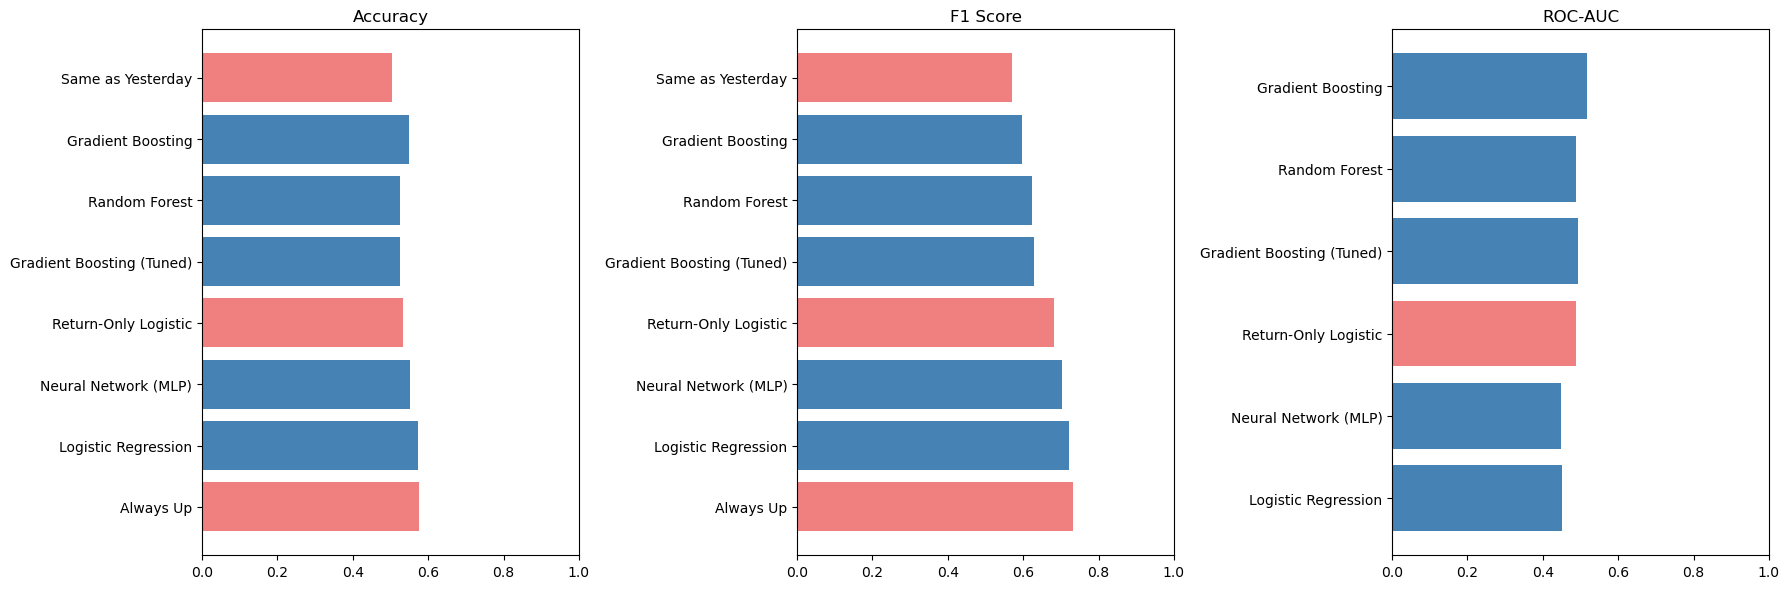
\includegraphics[width=\textwidth]{fig_model_comparison.png}
    \caption{Model comparison across three metrics. Red bars = baselines, blue bars = trained ML models.}
    \label{fig:comparison}
\end{figure}

\subsection{ROC Curves}

Figure~\ref{fig:roc} shows the ROC curves for all models that produce probability outputs. Most curves cluster near the diagonal, reflecting the inherent difficulty of daily market direction prediction. Gradient Boosting shows the best separation from the diagonal.

\begin{figure}[H]
    \centering
    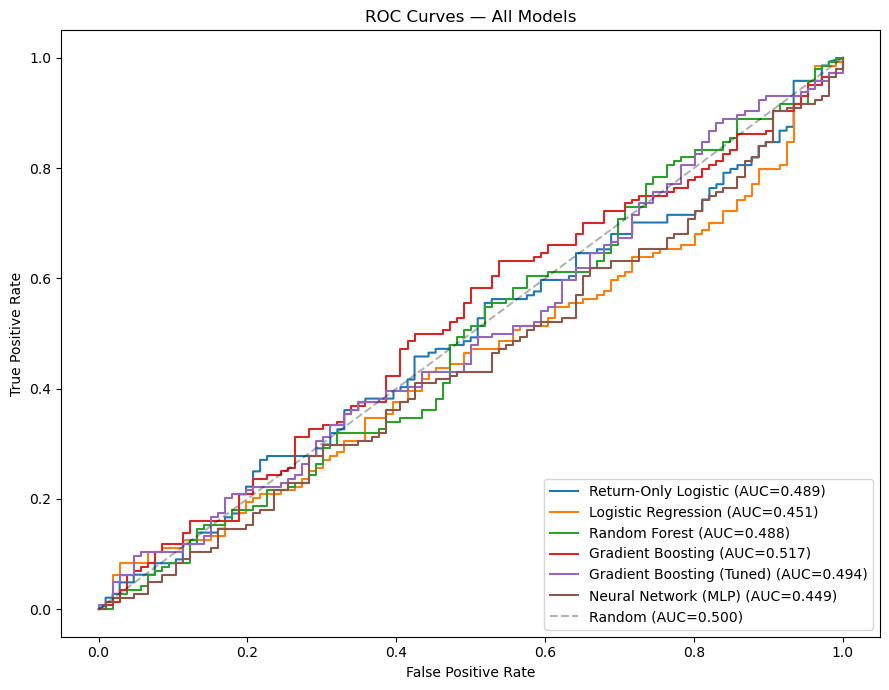
\includegraphics[width=0.75\textwidth]{fig_roc_curves.png}
    \caption{ROC curves for all probability-producing models. The dashed diagonal represents random guessing (AUC = 0.500). Gradient Boosting achieves the highest AUC at 0.517.}
    \label{fig:roc}
\end{figure}

\subsection{Feature Importance}

Figure~\ref{fig:importance} shows the top 15 features ranked by Random Forest importance. The VIX Close, Bollinger Band percent, and short-term volatility measures dominate, suggesting the model relies heavily on volatility-related signals.

From the Logistic Regression coefficients, the top features by absolute magnitude are: BB\_pct (0.757), SMA5\_vs\_SMA20 ($-$0.691), Lag\_1 ($-$0.571), VIX\_Close ($-$0.524), and Close\_vs\_SMA20 ($-$0.488).

\begin{figure}[H]
    \centering
    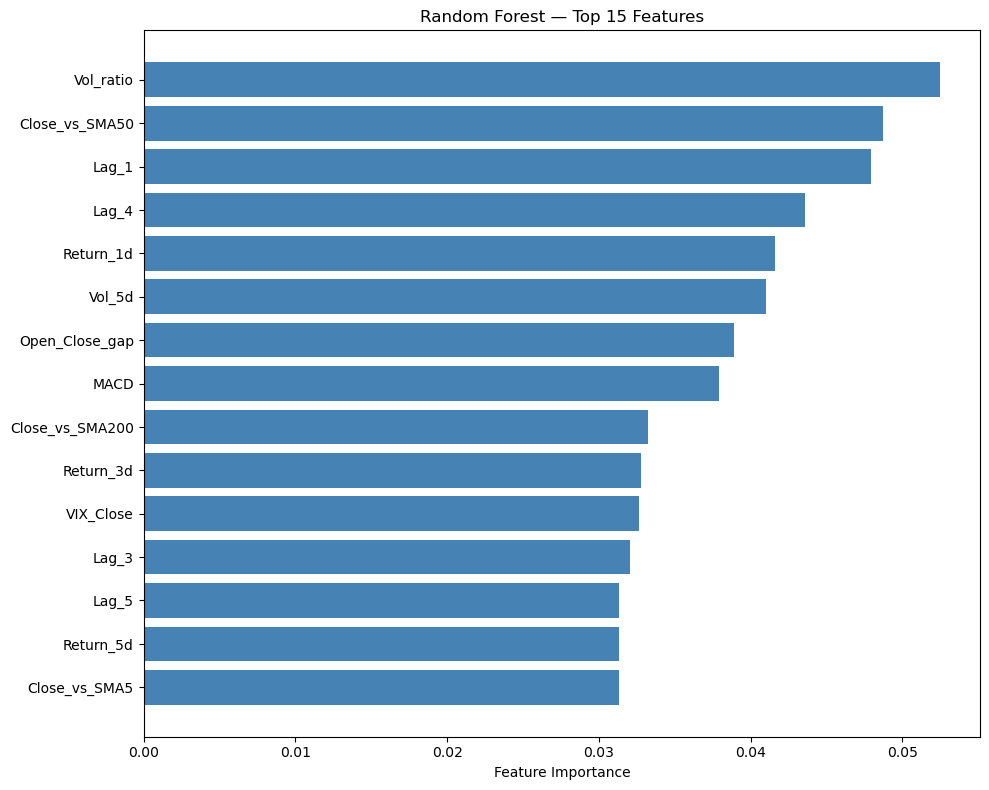
\includegraphics[width=0.75\textwidth]{fig_rf_importance.png}
    \caption{Top 15 features by Random Forest importance. Volatility-related features (VIX, Vol\_5d, BB metrics) rank highest.}
    \label{fig:importance}
\end{figure}

\subsection{Neural Network Training}

The neural network was trained with early stopping and converged at epoch 24. Figure~\ref{fig:nn} shows the training loss and validation F1 curves.

\begin{figure}[H]
    \centering
    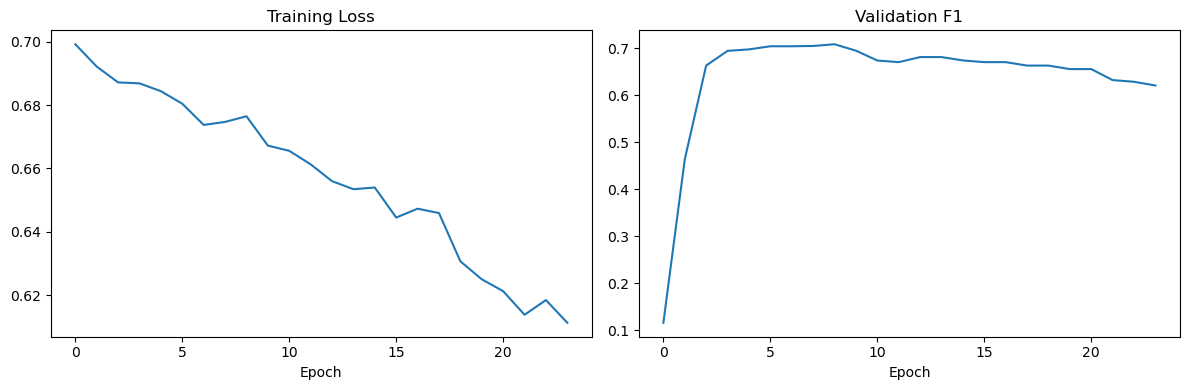
\includegraphics[width=0.85\textwidth]{fig_nn_training.png}
    \caption{Neural network training curves. Left: BCE training loss. Right: validation F1 score. Early stopping triggered at epoch 24 with a best validation F1 of 0.656.}
    \label{fig:nn}
\end{figure}

% ===================================================================
\section{Error Analysis}
\label{sec:error}

We analyze the Tuned Gradient Boosting model's predictions on the test set across different market regimes.

\subsection{Performance by Market Regime}

Table~\ref{tab:regimes} breaks down accuracy by VIX level, trend direction, and realized volatility.

\begin{table}[H]
\centering
\caption{Test accuracy by market regime (Tuned Gradient Boosting).}
\label{tab:regimes}
\begin{tabular}{llcc}
\toprule
\textbf{Regime} & \textbf{Condition} & \textbf{Accuracy} & \textbf{Days} \\
\midrule
High VIX     & VIX $>$ 17.2    & 0.5840 & 125 \\
Low VIX      & VIX $\leq$ 17.2 & 0.4640 & 125 \\
\midrule
Uptrend      & Close $>$ SMA50   & 0.5027 & 187 \\
Downtrend    & Close $\leq$ SMA50 & 0.5873 & 63  \\
\midrule
High Volatility & Vol\textsubscript{20d} $>$ 0.00824 & 0.5760 & 125 \\
Low Volatility  & Vol\textsubscript{20d} $\leq$ 0.00824 & 0.4720 & 125 \\
\bottomrule
\end{tabular}
\end{table}

Key findings from the regime analysis:

\begin{itemize}
    \item The model performs \textbf{significantly better during high-VIX periods} (58.4\%) than low-VIX (46.4\%). This makes sense: high VIX often signals sharper directional moves that are easier to predict, while low-VIX calm markets have more random noise.

    \item Similarly, \textbf{high realized volatility} periods yield 57.6\% accuracy vs.\ only 47.2\% during calm periods.

    \item The model is \textbf{more accurate during downtrends} (58.7\%) than uptrends (50.3\%). This could reflect the fact that downtrends tend to be driven by identifiable macro signals (VIX spikes, yield moves), while uptrends in 2025 were more gradual and harder to time on a daily basis.
\end{itemize}

\subsection{Monthly Accuracy}

Figure~\ref{fig:monthly} shows the model's accuracy broken down by month across the 2025 test period. Performance varies significantly---some months are well above the 50\% random-guess baseline while others fall below.

\begin{figure}[H]
    \centering
    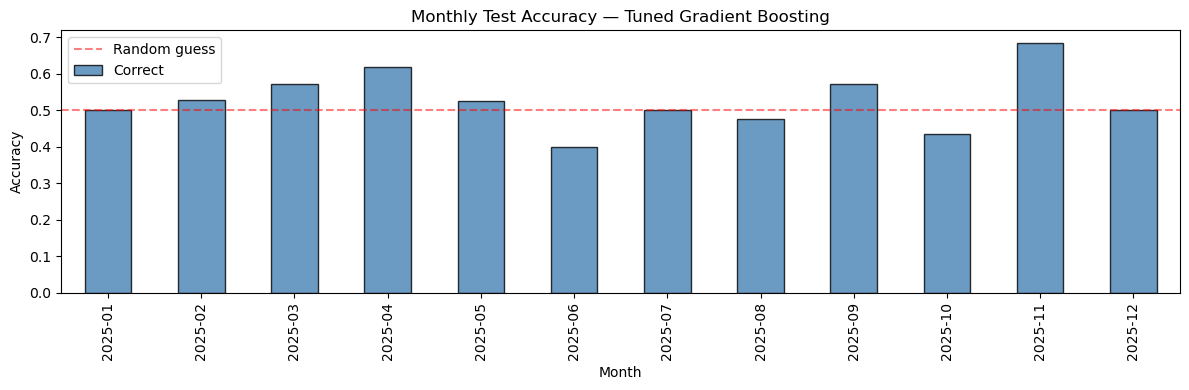
\includegraphics[width=\textwidth]{fig_monthly_accuracy.png}
    \caption{Monthly test accuracy for the Tuned Gradient Boosting model. Red dashed line = 50\% random guess. Performance varies across months, reflecting changing market conditions.}
    \label{fig:monthly}
\end{figure}

\subsection{Confusion Matrix}

Figure~\ref{fig:cm} shows the confusion matrix for the Tuned Gradient Boosting model. Out of 250 test days, the model correctly predicted 30 down days and 101 up days, while making 76 false positive errors (predicted up, went down) and 43 false negative errors (predicted down, went up).

\begin{figure}[H]
    \centering
    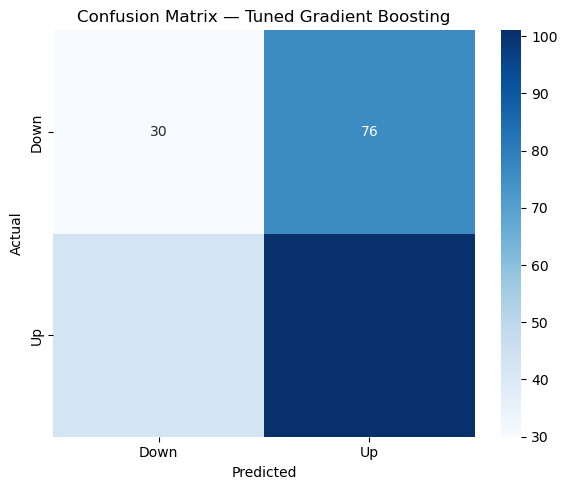
\includegraphics[width=0.45\textwidth]{fig_confusion_matrix.png}
    \caption{Confusion matrix for Tuned Gradient Boosting on the test set.}
    \label{fig:cm}
\end{figure}

\subsection{Prediction Timeline}

Figure~\ref{fig:timeline} overlays the model's predictions onto the actual S\&P 500 price during the test period. Green dots indicate correct predictions, red dots indicate errors. The bottom panel shows cumulative accuracy over time.

\begin{figure}[H]
    \centering
    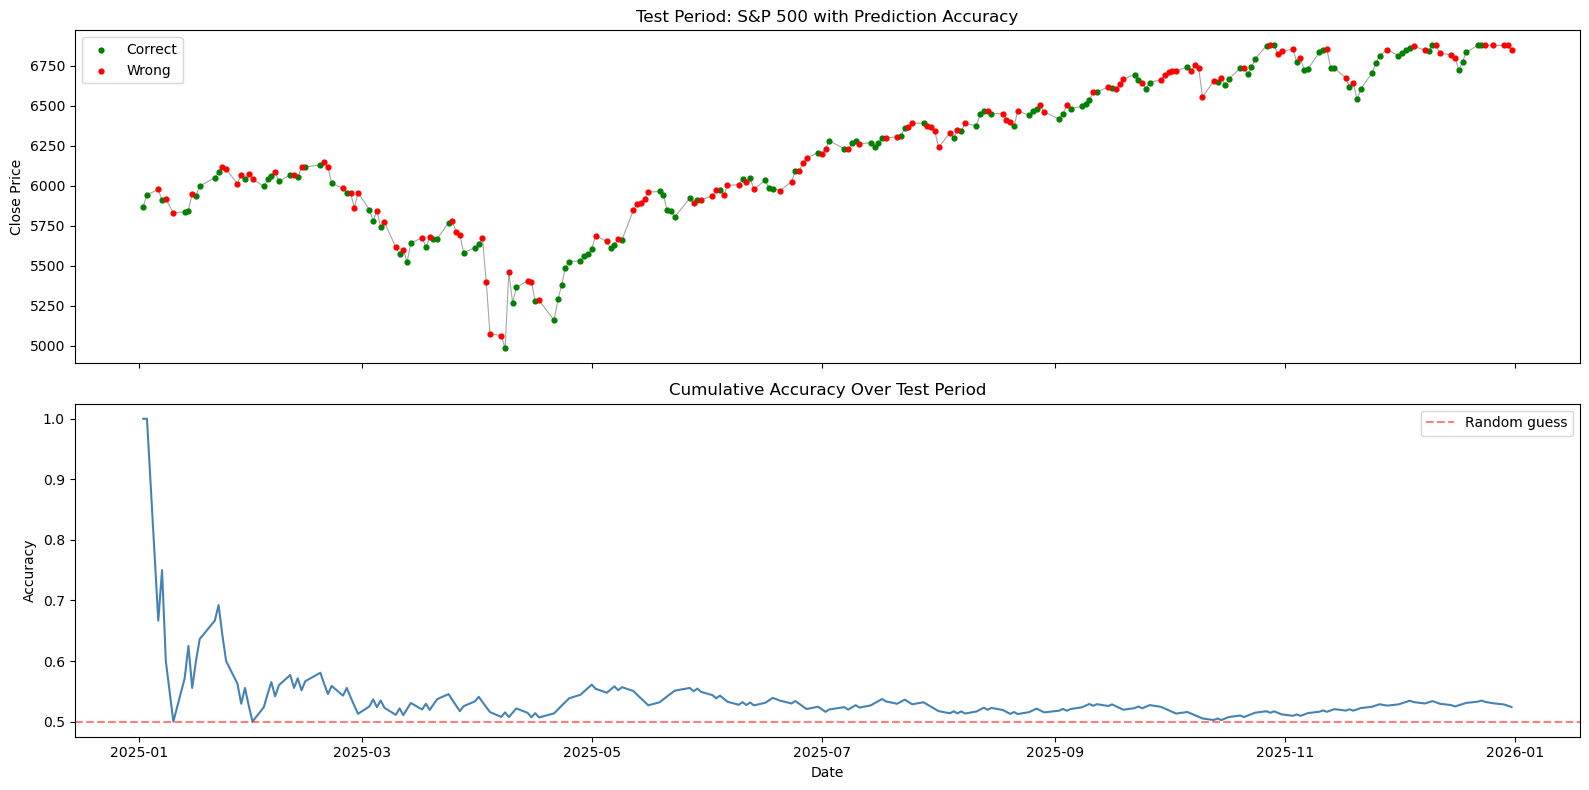
\includegraphics[width=\textwidth]{fig_prediction_timeline.png}
    \caption{Top: S\&P 500 test period with correct (green) and incorrect (red) predictions. Bottom: cumulative accuracy over time, converging near the final accuracy of 52.4\%.}
    \label{fig:timeline}
\end{figure}

% ===================================================================
\section{Discussion}
\label{sec:discussion}

\subsection{Key Findings}

\begin{itemize}
    \item The \textbf{Always-Up baseline is deceptively strong} (57.6\% accuracy, 0.731 F1) due to the market's upward drift during the test period. This underscores why raw accuracy and F1 alone are insufficient---ROC-AUC and precision provide more informative comparisons.

    \item \textbf{Gradient Boosting} is the only model to achieve ROC-AUC above 0.50 (0.517) and precision above 61\%, suggesting it learns some genuine directional signal rather than defaulting to ``always up.''

    \item \textbf{Linear and neural models} (Logistic Regression, MLP) tend to collapse toward always predicting ``up,'' likely because the slight class imbalance (57.6\% up) makes this the path of least resistance during training.

    \item \textbf{Walk-forward tuning} reveals high variance across folds (std up to $\pm$0.10), highlighting the instability of any learned signal---what works in one market period may not transfer to another.

    \item \textbf{Regime analysis} shows that models work better when the market is volatile or in a downtrend, suggesting the features capture ``fear'' signals (VIX spikes, volatility jumps) more effectively than ``complacency'' signals during calm uptrends.
\end{itemize}

\subsection{Limitations}

\begin{itemize}
    \item \textbf{Dataset size}: Four years of daily data yields only 794 usable samples after warmup, limiting the complexity of models we can reliably train. The neural network in particular likely suffers from this.

    \item \textbf{Regime shifts}: The model is trained on 2022--2024 (which includes a bear market in 2022 and a strong bull run in 2023--2024) and tested on 2025. If market dynamics shifted significantly, performance degrades.

    \item \textbf{Feature set}: We use only four external data sources. Incorporating sentiment data (news, social media), sector-level indicators, or higher-frequency data could improve performance.

    \item \textbf{Transaction costs}: We evaluate directional accuracy only. A real trading strategy would need to account for transaction costs, slippage, and position sizing.

    \item \textbf{Class imbalance}: With 57.6\% up days in the test set, the models are incentivized to predict ``up'' frequently, inflating recall at the expense of precision. Techniques like class weighting or threshold calibration could help balance this.
\end{itemize}

% ===================================================================
\section{Conclusion}
\label{sec:conclusion}

We built a complete pipeline for predicting S\&P 500 next-day direction, from raw data ingestion through feature engineering, model training, hyperparameter tuning with walk-forward validation, and regime-based error analysis. Multiple model families were compared against meaningful baselines using time-aware evaluation on 250 held-out trading days.

The results demonstrate that daily market direction is extremely noisy---even our best model (Gradient Boosting, ROC-AUC = 0.517) only marginally exceeds random chance. However, the regime analysis reveals a more nuanced story: models perform meaningfully better during high-volatility and high-VIX periods (58.4\% accuracy vs.\ 46.4\% in calm markets), suggesting that ML can identify directional signals when the market is moving sharply but struggles with the random noise of calm trading days.

Tree-based ensembles, particularly Gradient Boosting, provide the best balance of precision and discriminative ability for this task. Future work could explore larger datasets, alternative feature sources (sentiment, options flow), and more sophisticated architectures (LSTMs, Transformers) to push performance further.

% ===================================================================
\section*{Division of Work}

\begin{itemize}
    \item \textbf{Eric Liu}: Data loading, data cleaning, feature engineering pipeline, exploratory data analysis, hyperparameter tuning, evaluation metrics computation, report writing.
    \item \textbf{Rithikesh Muddana}: Baseline models, logistic regression, random forest implementation, all visualizations (heatmaps, ROC curves, feature importance, prediction timeline), error analysis, data alignment documentation.
    \item \textbf{Shared}: Gradient boosting, neural network, chronological split design, code review, debugging.
\end{itemize}

% ===================================================================
\section*{Repository}

All code is available at: \url{https://github.com/erizeli/S-P-500-Predictor}

\end{document}
